Primero describimos la estructura de datos para una de las aplicaciones más simples de esta idea, luego mostramos cómo generalizarla para resolver algunos problemas.

Dado un arreglo $a[0 \dots n-1]$, implemente una estructura de datos que permita encontrar la suma de los elementos $a[l \dots r]$  para arbitrarios $l$ y $r$.

La idea básica de  la descomposición de raíz cuadrada es preprocesamiento. Dividiremos el arreglo $a$ en bloques de longitud aproximadamente $\sqrt n$, y por cada bloque $i$ precalcularemos la suma de elementos en $b[i]$. Por ejemplo, una matriz de 16 elementos dividirse en bloques de 4 elementos de la siguiente manera:

% TODO: \usepackage{graphicx} required
\begin{figure}[h!]
	\centering
	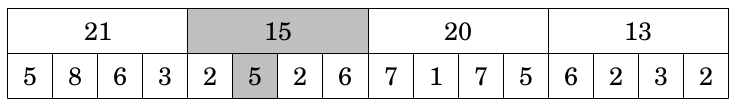
\includegraphics[width=0.7\linewidth]{img/srt_descomposition1}
	\label{fig:srtdescomposition1}
\end{figure}


Podemos asumir que tanto el tamaño del bloque como el número de bloques son iguales a $\sqrt n$  redondeado:

$$ s = \lceil \sqrt n \rceil $$

Luego el arreglo $a$ se dividirá en bloques de la siguiente manera:

$$ \underbrace{a[0], a[1], \dots, a[s-1]}_{\text{b[0]}}, \underbrace{a[s], \dots, a[2s-1]}_{\text{b[1]}}, \dots, \underbrace{a[(s-1) \cdot s], \dots, a[n-1]}_{\text{b[s-1]}} $$

El último bloque puede tener menos elementos que los demás (si $n$ no un múltiplo de $s$ ), no es importante para la discusión (como se puede manejar fácilmente). Por lo tanto, por cada bloque $k$ , conocemos la suma de elementos en él $b[k]$.

$$ b[k] = \sum\limits_{i=k\cdot s}^{\min {(n-1,(k+1)\cdot s - 1})} a[i] $$

Por lo tanto, hemos calculado los valores de $b[k]$ en O($n$). ¿Cómo pueden ayudarnos a responder a cada consulta $[l,r]$ ? Observe que si el intervalo $[l, r]$ es lo suficientemente largo, contendrá varios bloques enteros, y para esos bloques podemos encontrar la suma de elementos en ellos en una sola operación. Como resultado, el intervalo $[l, r]$ contendrá partes de sólo dos bloques, y tendremos que calcular la suma de elementos en estas partes trivialmente.

Por lo tanto, para calcular la suma de elementos en el intervalo $[l, r]$  sumar los elementos de las dos partes:  $a[l\dots (k + 1)\cdot s-1]$ y $a[p\cdot s\dots r]$ , y sumar los valores $b[i]$ en todos los bloques de $k + 1$ to $p-1$. Cuando $ K = P $, es decir, $ L $ y $ R $ pertenecen al mismo bloque, la fórmula no se puede aplicar y la suma debe calcularse de manera trivial.

% TODO: \usepackage{graphicx} required
\begin{figure}[h!]
	\centering
	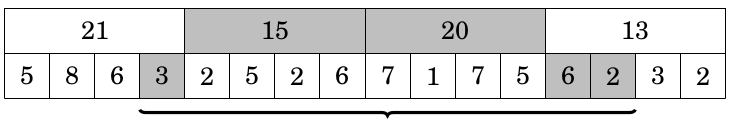
\includegraphics[width=0.7\linewidth]{img/srt_descomposition2}
	\label{fig:srtdescomposition2}
\end{figure}

Este enfoque nos permite reducir significativamente el número de operaciones.De hecho, el tamaño de cada parte no es la longitud del bloque $s$, y el número de bloques en la suma no excede de $s$.Dado que se elige a $s \approx \sqrt n$, el número total de operaciones necesarias para encontrar la suma de elementos en el intervalo $[l, r]$ es $O(\sqrt n)$.
